\documentclass[convert={size=420x380}]{standalone}
\usepackage[utf8]{inputenc}
\usepackage{tikz}
\usetikzlibrary{calc, decorations.markings}
\usepackage{siunitx}
\sisetup{locale=FR, per-mode=symbol}

\begin{document}
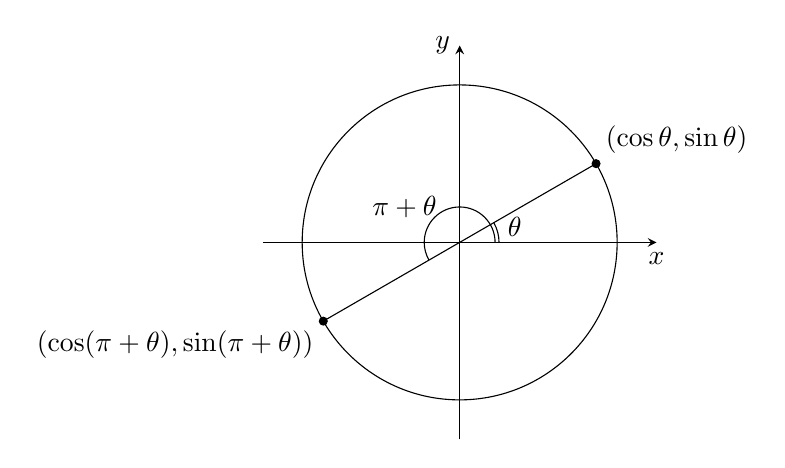
\begin{tikzpicture}[>=stealth]
  %\clip (-1.2, -1.6) rectangle (5.75, 2.7);
  \def\radius{2}
  \def\angle{30}
  \coordinate (O) at (0, 0);
  \coordinate (A) at ($(O) + (\angle:\radius)$);
  \coordinate (B) at ($(O) + (180+\angle:\radius)$);
  \draw (O) circle(\radius);
  \draw[->] (-\radius - 0.5, 0) -- (\radius + 0.5, 0) node[below] {$x$};
  \draw[->] (0, -\radius - 0.5) -- (0, \radius + 0.5) node[left] {$y$};
  \node[anchor=south west] at (A) {$(\cos\theta, \sin\theta)$};
  \draw[fill=black] (A) circle (0.05);
  \node[anchor=north east] at (B) {$(\cos(\pi+\theta), \sin(\pi+\theta))$};
  \draw[fill=black] (B) circle (0.05);
  \draw ($(O) + (0.5, 0)$) arc (0:\angle:0.5);
  \node at (0.7, 0.2) {$\theta$};
  \draw (O) -- (A);
  \draw ($(O) + (0.45, 0)$) arc (0:180+\angle:0.45);
  \node at (-0.7, 0.45) {$\pi + \theta$};
  \draw (O) -- (B);
\end{tikzpicture}
\end{document}

